%CHANGE FIGURE NO AGENT FLOCKING

\section{Results}
\subsection{No agent}
To provide a baseline for what flocking behaviour looks like figure \ref{fig:NoAgentFlocking} demonstrates flocking with constant gains for each step. the flocking can be seen to occur as drones are in proximity to each other and all drones are arriving at their individual destinations.

\begin{figure}[h]
  \begin{center}
    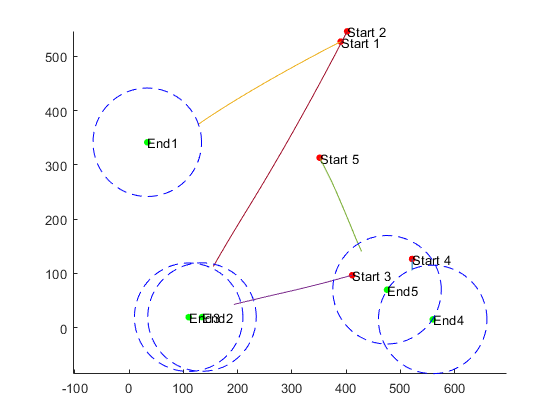
\includegraphics[width=0.4\textwidth]{figures/NoAgent.png}
    \end{center}
    \caption{No agent Flocking}
    \label{fig:NoAgentFlocking}
\end{figure}

\subsection{Agent training}
During the training, the agents would behave in a stochastic fashion to facilitate exploration. The training was stopped once a satisfactory average reward was achieved and the subsequent agents were saved.


\begin{figure}[h]
  \begin{center}
    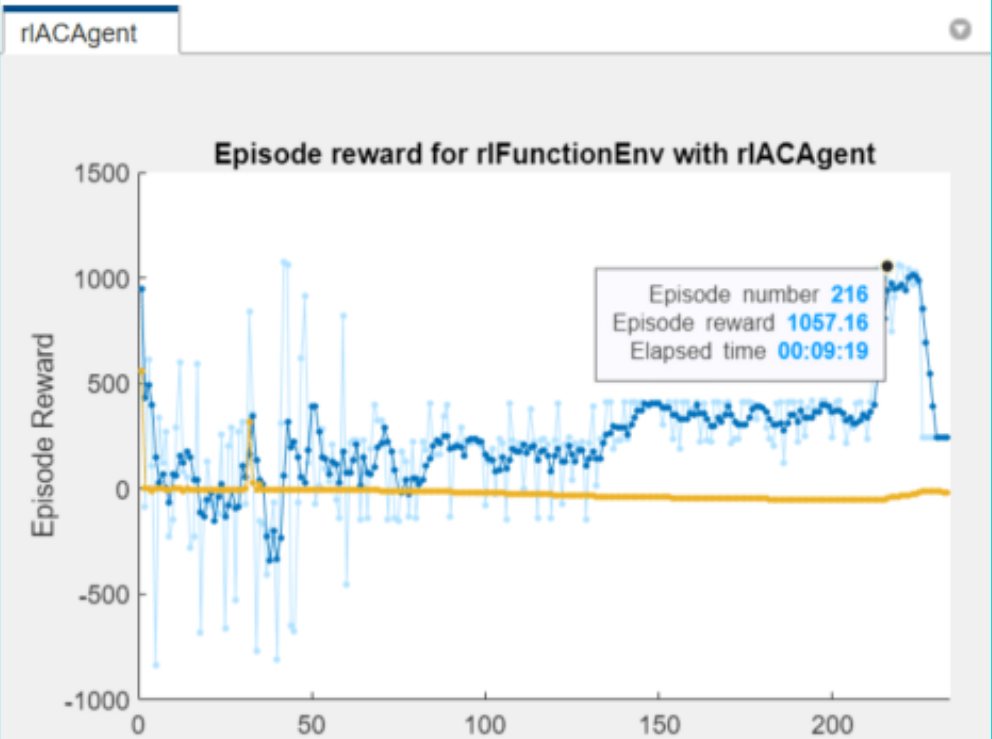
\includegraphics[width=0.4\textwidth]{figures/TrainingData.PNG}
    \end{center}
    \caption{Agent Training}
    \label{fig:Agent Training}
\end{figure}

Figure \ref{fig:Agent Training} demonstrates this training where 3 values are shown: episode reward, an average taking into account the last 5 episodes and the Q0 estimated reward. The average reward, calculated over the last 5 steps, steadily increases as the agent performs more episodes. The agent learns steadily until it reaches a certain amount of episodes and suddenly loses all its learned behaviour. This is a common issue in reinforcement learning classified as "catastrophic forgetting"\cite{cat1}. This might be corrected by varying the learning rate once a certain agent is achieved. This would mean the agent would have a more robust policy function although learn slower.

\subsection{Trained agent}
Once trained the agent behaves in a deterministic way as it has established the optimal policy function. This means for every state input the agent has a definite action to perform. The simulation is then repeatable as there is a definite action for every state. 

\begin{figure}[h]
  \begin{center}
    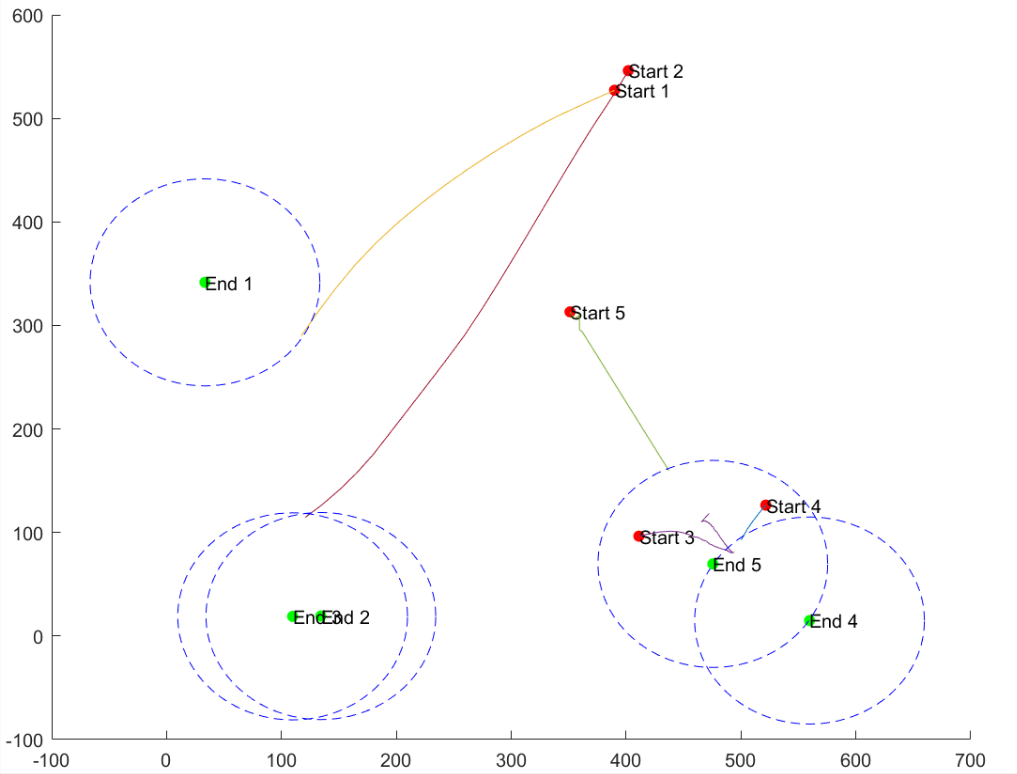
\includegraphics[width=0.6\textwidth]{figures/TrainedAgent.PNG}
    \end{center}
    \caption{Trained Agent}
    \label{fig:TrainedAgentFlocking}
\end{figure}

\subsection{Emergent Behaviour}
Emergent behaviour is a qualitative analysis that is useful in understanding how the reward affects agent behaviour. If certain undesirable behaviours emerge this is a sign that the reward function is promoting the wrong actions. From the trained agent’s performance in figure \ref{fig:TrainedAgentFlocking} some useful behaviours arise as well as some problematic behaviours:

\begin{itemize}
\item
Flocking is achieved which shows drones 1 and 2 arriving at designated locations from sides that benefit both members, this might be useful if multiple drones need to deliver packages but also avoid certain areas. 

\item
Some drones are not arriving at their destination which is a definite example of a scenario that is a detriment to the system. Drone 3 is choosing to flock with drones 4 and 5 rather than arrive at the destination. 

\end{itemize}
\clearpage
\section{Discussion}
The actions that the agent can perform are what determine how the agent controls the system. Providing the agent with a guidance system constrains the possibilities of actions it can take which has positive and negative influences on the system:\vspace{0.2cm}

\noindent
\textbf{+} The agent can learn quickly as there are fewer possible actions.\\

\noindent
\textbf{-}The agent is constrained to certain motions and is not given enough degrees of freedom the system lacks controllability.\cite{con2}\hfill\vspace{0.2cm}

\noindent
Since the first publication in 1987\cite{boid0}, the boid flocking behaviour has been iterated upon to provide the agent with the ability to learn new behaviours. These include having different perception radii for separation, alignment and cohesion, limiting the field of view of boids and allowing for flock leaders.\cite{boid1} These are just some examples of model variation that are possible. The application would be used to design the model. In the case of drones, lidar or some such sensor might be to detect the relative and heading of other UAVs. The simulation in this project uses a very simplistic model of the world. To reach further conclusions it would be desirable to further elaborate on the model.
The reward function here focuses on only 2  characteristics: The position of the drone and the number of steps  taken. The emergent behaviour exhibited by the drone is limited by this. Additional factors could be taken into account especially if the model representation expanded such as the power used to create a path.
In this case, the reward function promotes drone flocking as well as arriving at individual destinations within a limited number of steps in any scenario. This simulation is in 2 dimensions, so the altitude is not considered. This would obviously play a role in deciding whether to flock if a drone is at a certain altitude or is descending towards its destination.\\
Positive emergent behaviour was achieved in some sense so to continue down this path it is important to establish why it is being successful and how the reward function and overall machine learning structure can be leveraged to further improve the algorithm.

\subsection{Improvements}
To further encourage the positive emergent behaviour as well as discourage the issues that arise multiple factors come into play

\subsubsection{Machine learning structure}

The structure of learning can affect the learning speed of the agent but also be used to determine the application of the agent. The current machine learning structure uses a centralised agent that controls n drones, providing a [5, N] gain matrix at each iteration step controlling the swarm. Instead of this a multi-agent structure can be defined where each agent controls a single drone. This would simulate a decentralised network which is better suited to a multi-vehicle system.

\begin{itemize}
    \item 
    The application could work with drones that are not in communication with each other if there is sufficient sensor information about other drones. This structure would also mean the number of drones would no longer affect the dimensions of action and state matrices creating a more generalised agent. 
    \item
    Learning speed would increase as a result of agents learning in parallel, as for a simulation with N drones N agents would be trained as opposed to 1. To go even further 
    \item
    Agents could be assessed individually rather than taking a weighted sum of the overall reward. Agents could be removed from every simulation and the best ones could be used to seed the next generation of agents. This would improve the learning rate as well.
\end{itemize}

\subsubsection{Environment}
In this case, the environment is simplistic. There are no obstacles included as well as very simple environmental dynamics. The system could be represented in 3D and additional environmental characteristics could be included such as:

\begin{itemize}
    \item Differentiation of quad-copter\cite{quad1} and fixed-wing\cite{fix1} dynamics could be introduced to find how this affects the way they interact with each other.
    
    
    
    \item Consider benefits of flocking for efficiency for fixed-wing UAVs \cite{fix1}.
    
    \item Consider prevailing winds making use of head and tailwind.
    
\end{itemize}

\subsubsection{Optimisation}
Optimising the simulation is important in reinforcement learning as the more episodes that can be performed the more the agent can optimise its policy function. Code refactoring could be achieved through:

\begin{itemize}
    \item 
    Inclusion of a Quad-tree\cite{ref1}, which is a programming technique that compresses spacial data limiting the number of checks that need to be done when calculating whether agents are close to one another.
    \item
    Making use of specialised hardware that is optimised for RL\cite{ref2}.
    \item
    Using open AI platform to produce a better reinforcement learning structure.\cite{AI}
\end{itemize}



\subsubsection{Reward Function}
Being the key cause for emergent behaviour the reward function can be changed to take into account more of the environment. This clearly benefits from more in-depth environmental dynamics. The function that is used in this scenario is specifically tailored for the specific range. The reward function could be altered in many ways depending on the intended application, here are some possibilities:

\begin{itemize}
    \item 
    Make reward for position relative to the range that it will be used to make more general emergent behaviour.
    
    \item
    Include altitude in the 3-dimensional environment
    
    \item Include additional penalty for position, namely no fly-zones \cite{res1}.
\end{itemize}

